% !TEX root =  ../report.tex
\section{Introduction}

\subsection{Evaluated Objective}
The purpose of the heuristic evaluation is to identify, evaluate and possibly solve problems that are present in the front-end design of the Talio application.

Evaluators will receive the design of the application, created using "Figma", an online tool used for mock-ups and prototyping the design of an application. The prototype is not functional - it is only composed of images which should resemble the front-end design of the application. Therefore, mock-ups used for this heuristics report are inserted:

\subsection{Evaluated Prototype}

\begin{figure}[H]
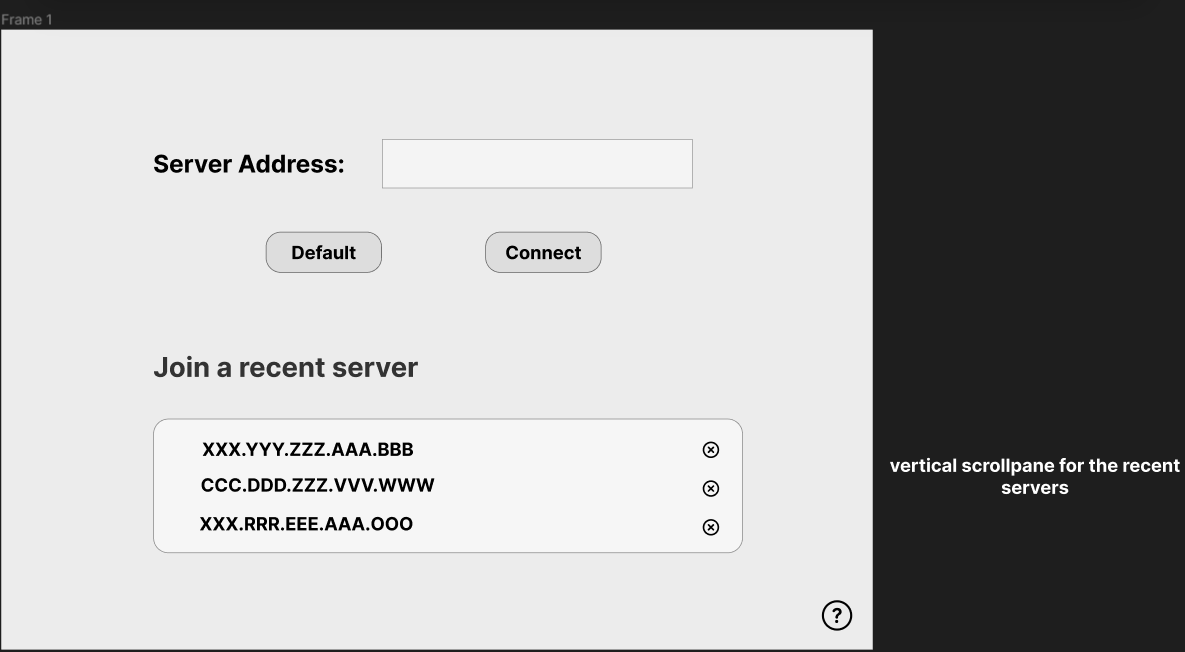
\includegraphics[width=5cm]{content/mockups/server_connect.png} 
\caption{Connect to server}
\end{figure}

The server connection frame is the first displayed thing when the application is started. Here the user can choose a custom server URL or proceed with the default option. If the provided URL is not valid then an error message is shown.

\begin{figure}[H]
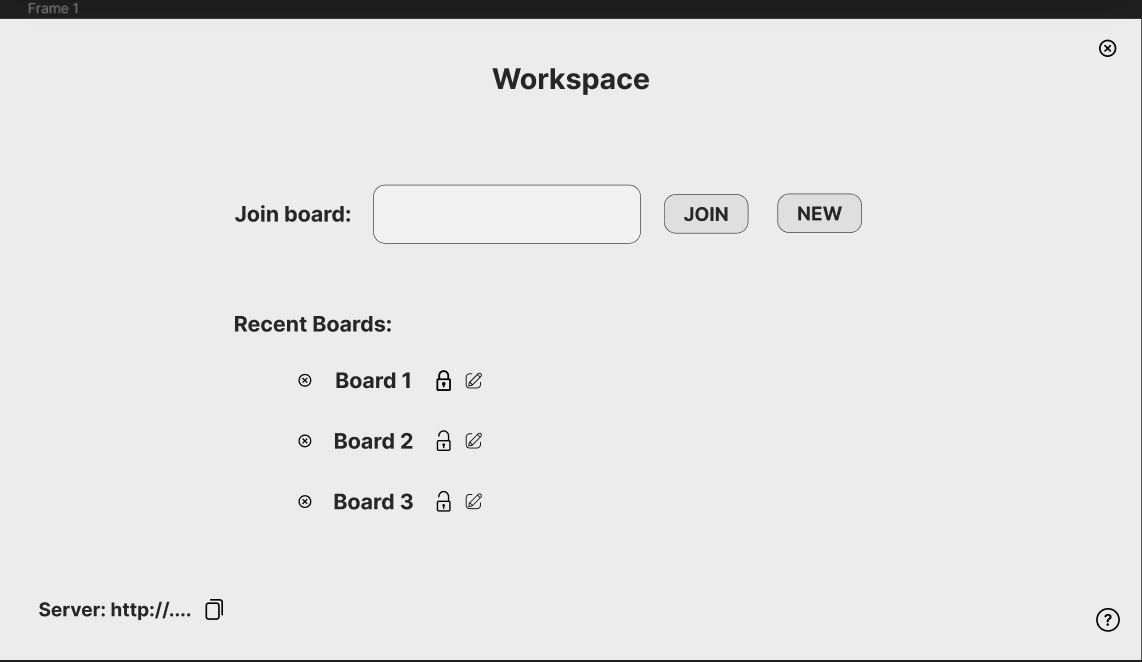
\includegraphics[width=5cm]{content/mockups/workspace.png} 
\caption{Workspace}
\end{figure}

Upon successful connection, the workspace frame is displayed. From here the user can choose to join a recent board, join new board or create one.

\begin{figure}[H]
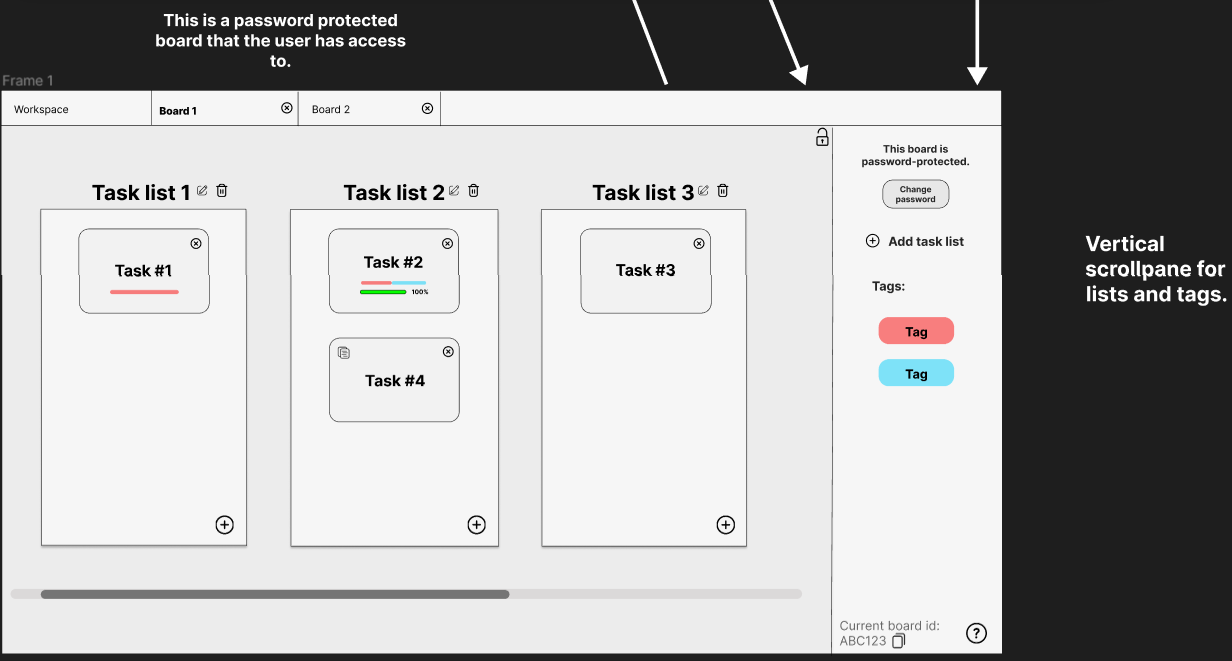
\includegraphics[width=5cm]{content/mockups/overview_frame_1.png} 
\caption{Password protected board with access to it}
\end{figure}

Boards can either be password protected or not, meaning that some boards require a password to be changed. Password is not required to view the board.

\begin{figure}[H]
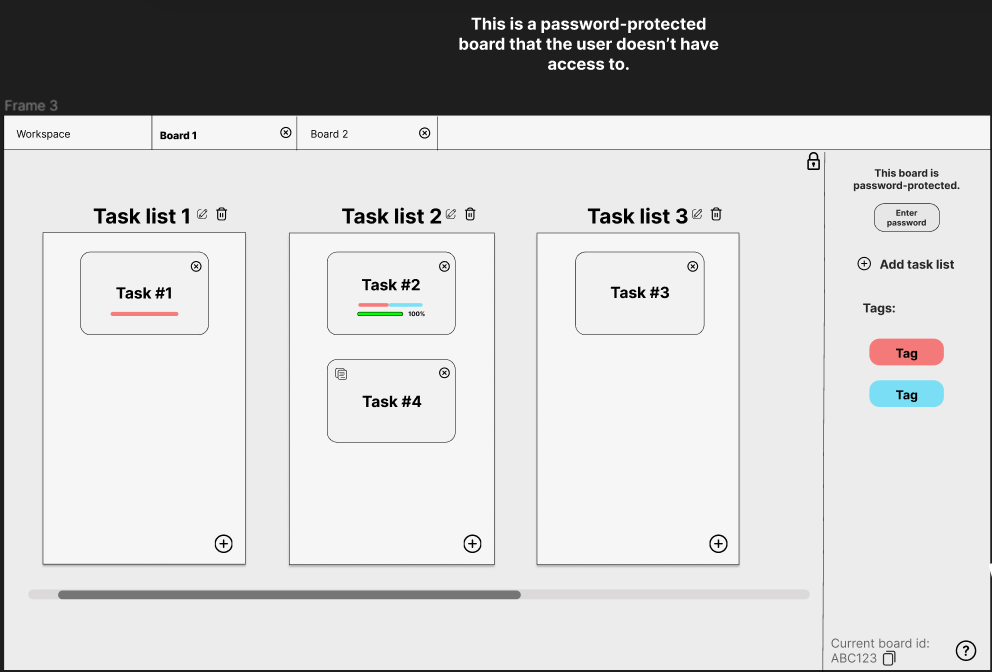
\includegraphics[width=5cm]{content/mockups/overview_frame_3.png} 
\caption{Password protected board without access to it}
\end{figure}

If the user wants to edit a board without entering the password. Then an error message shows up.

\begin{figure}[H]
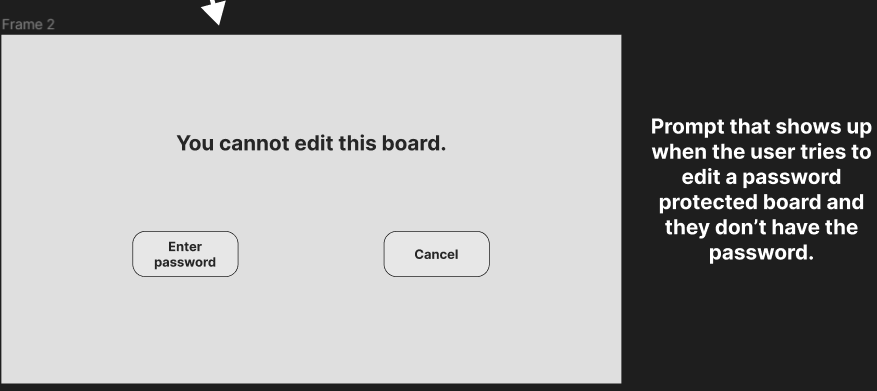
\includegraphics[width=5cm]{content/mockups/overview_frame_2.png} 
\caption{Error message}
\end{figure}

This error message informs the user that they do not write permissions unless they provide a valid password.

\begin{figure}[H]
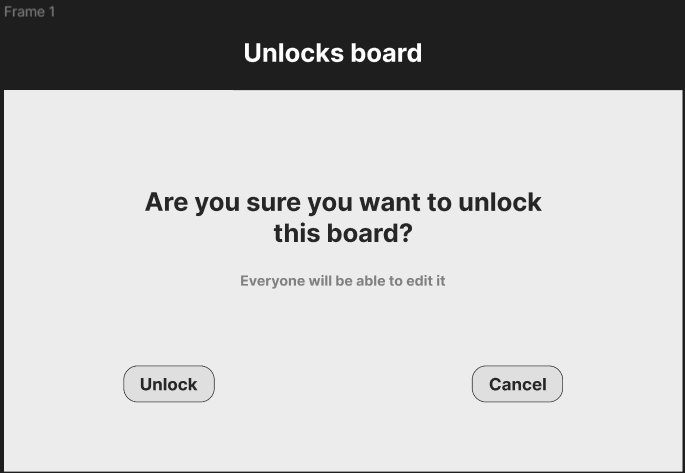
\includegraphics[width=5cm]{content/mockups/password_frame_1.png} 
\caption{Remove password}
\end{figure}

Of course, boards can be unlocked. This may sound ambiguous, however, unlocking a board means removing its password and making it available to be edited by everyone.

\begin{figure}[H]
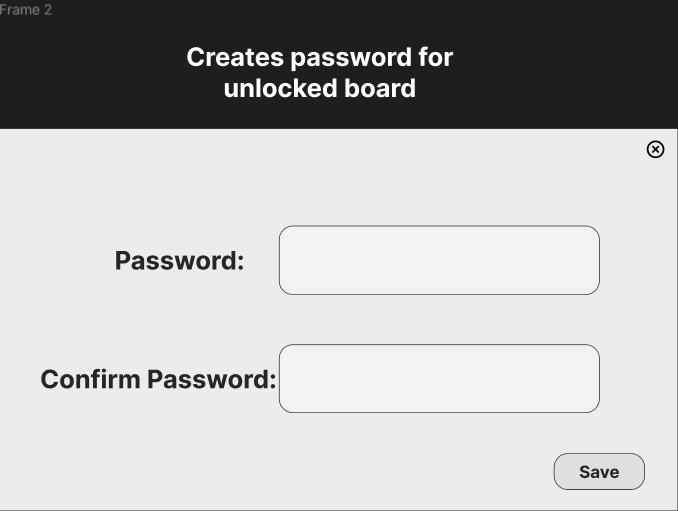
\includegraphics[width=5cm]{content/mockups/password_frame_2.png} 
\caption{Create password}
\end{figure}

Respectively, boards can be locked via the same principle. The only thing a user needs to do is create a password to lock the board.

\begin{figure}[H]
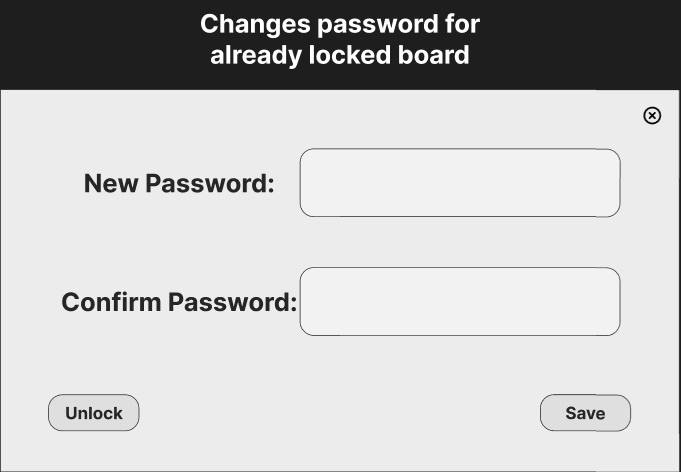
\includegraphics[width=5cm]{content/mockups/password_frame_3.png} 
\caption{Change password}
\end{figure}

If the user desires to change the password of the board, that is also possible

\begin{figure}[H]
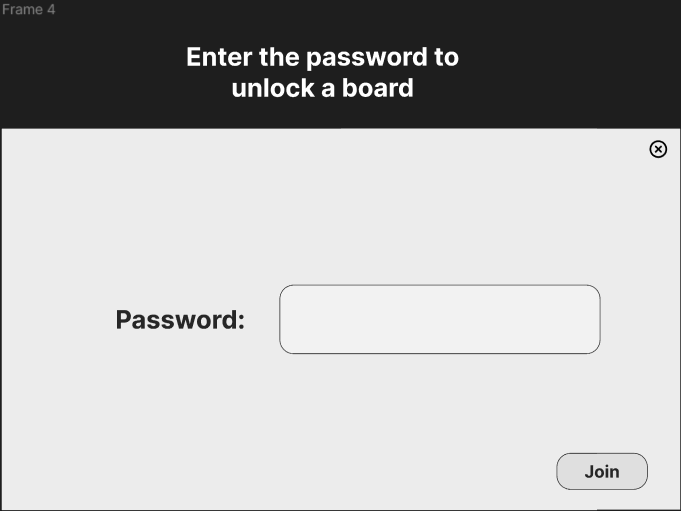
\includegraphics[width=5cm]{content/mockups/password_frame_4.png} 
\caption{Unlock board}
\end{figure}

Of course, boards can be accessed and edited without removing the password. However, the rights to edit a board remain only while the user has the board opened. Should the user close the board, they need to unlock it again via password.

\begin{figure}[H]
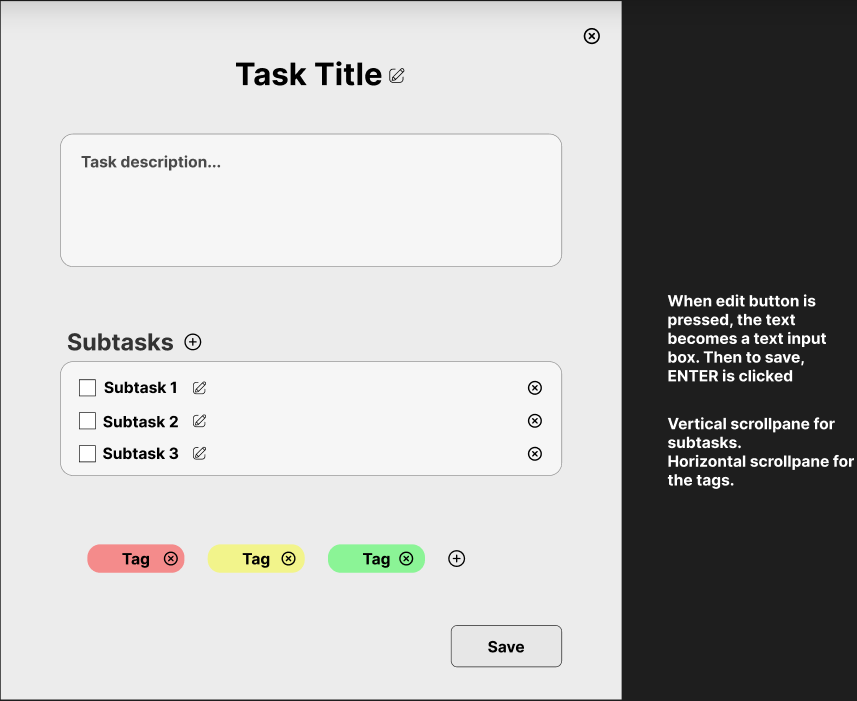
\includegraphics[width=5cm]{content/mockups/task_view_frame_1.png} 
\caption{Task view}
\end{figure}

Whenever a task is clicked on, a popup is shown which enables the user to edit the task. The design is simple and allows the user to change the title, description, tags and sub tasks of the selected task.

\begin{figure}[H]
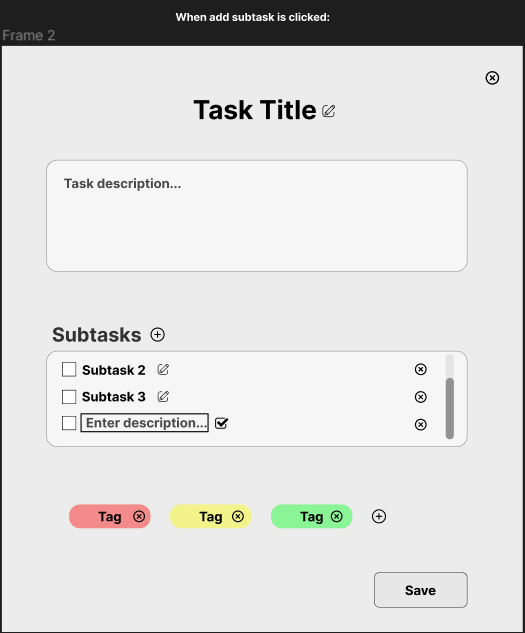
\includegraphics[width=5cm]{content/mockups/task_view_frame_2.png} 
\caption{Editing sub tasks view}
\end{figure}

Furthermore, the description of the sub tasks can be changed via the edit button next to them. Upon clicking the edit button, it enables the sub task to be edited and saves the sub task if clicked once again.

\begin{figure}[H]
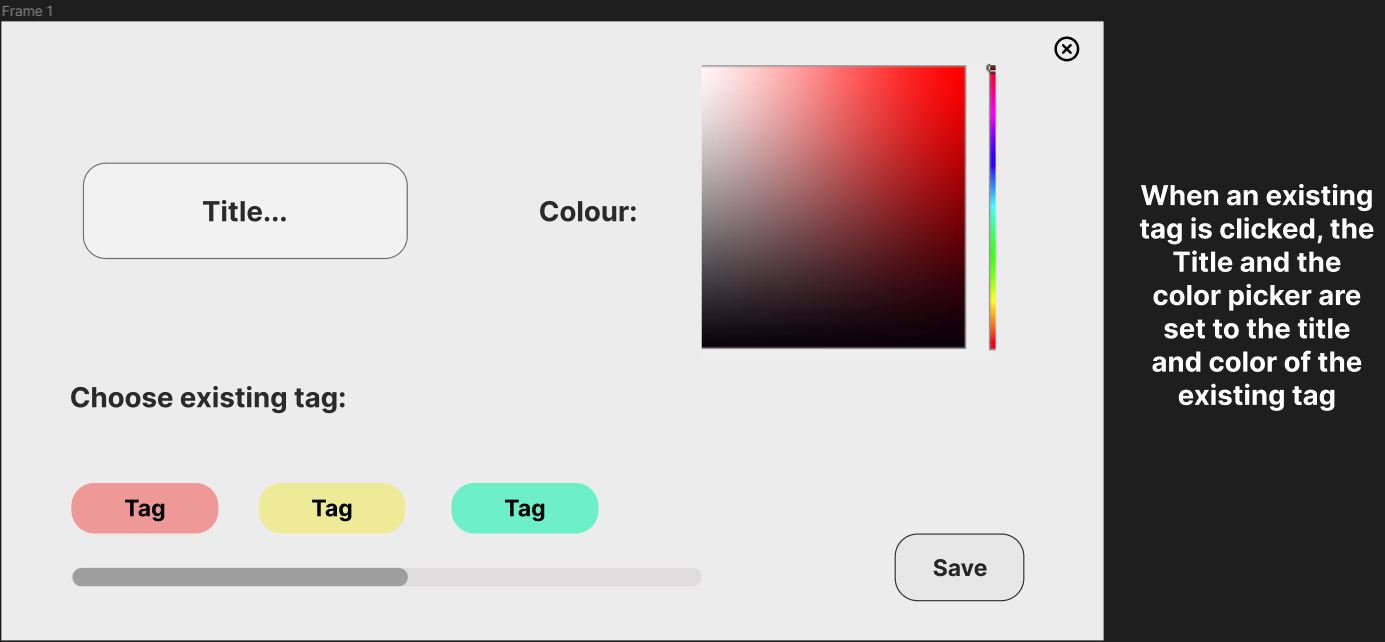
\includegraphics[width=5cm]{content/mockups/edit_tag.png} 
\caption{Add/Edit tag}
\end{figure}

Tags can be created and edited. The color is chosen via the color wheel. Moreover, existing tags are displayed from which the user can choose.